\documentclass[11pt]{article}
\usepackage{geometry}                
\geometry{letterpaper}
\usepackage[]{graphicx}
\usepackage{amssymb}
\usepackage{amsmath}
\usepackage{amsthm}
\usepackage{fancyhdr}
\usepackage{amsthm}
\usepackage[english]{babel}

\title{Exploiting Math.expm1(-0) in v8 TurboFan JIT Compiler}
\author{Ryan Torok, Sara McFearin, Michael Jarrett, Rachel Shi}
\date{December 7, 2019}
\begin{document}
\maketitle
\section{Introduction}
Browser bugs are difficult to find, but they appear to be prevalent across all four major browser
engines. In recent years most of the focus has been on bugs in the JavaScript Just-in-Time (JIT)
compilers. Improper optimization can often lead to a memory corruption exploit which allows the
attacker to take control of the victim's browser and begin executing aribtrary code on the victim's
machine, making browser bugs a popular target for cybercriminals who run botnets, ransomware scams,
and more. Although it is not uncommon for compilers to contain bugs in their large codebases,
browser JIT compilers are unique in the sense that they must deal with adversarially chosen code. In
a normal pre-compilation setting, if a compiler bug is found, programmers simply won't write code
that triggers the bug for sake of security. However, in browsers, the compiler runs on the user's
machine, and if a browser JIT compiler bug is found, attackers will intentionally ship code which
triggers the bug in order to take over the user's machine. 

With this in mind, it seems like we will be playing an infinite game of Whack-a-mole with browser
JavaScript engines, but new techniques have risen in recent years to make bug elimination faster,
most notably Fuzzing. Fuzzing is a technique which originated in image encoding protocols, where a
penetration tester will pass random binary inputs to the protocol attempting to cause a crash. With
some modifications based on knowledge of how browser JITs create a graph of a code segment,
penetration testers can write automated tools which generate random JavaScript code inputs which
look somewhat interesting. The most popular of these tools is called \textit{Fuzzily}, which has
already found a plethora of bugs in the JavaScript engines for all four major web browsers.

\section{The Bug}
\begin{figure}
	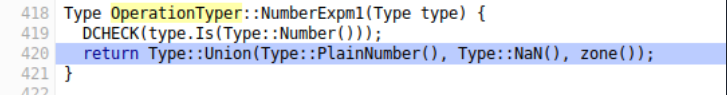
\includegraphics[width=\linewidth]{typer.png}
	\caption{The buggy return type declaration for Math.expm1() in operation-typer.cc}
  \label{fig:typer}
\end{figure}	
We will focus now on one of these bugs in particular. The TurboFan JIT compiler used by v8, the
JavaScript engine for the Chrome and Chromium web browsers, was exploited in 2018 using an edge case
with the function \texttt{Math.expm1()}, which computes $e^x -1$ for argument $x$.  Specifically, if
we evaluate \texttt{Math.expm1(-0)}, this should produce the value -0.  However, the TurboFan JIT
lists the return types for this function as a union of the \texttt{PlainNumber} type and NaN. This
union includes all values of a 64-bit floating point number, except -0. V8 defines this behavior
using a special table in typer.cc and operation-typer.cc. The code from the latter is shown in
Figure \ref{fig:typer}. The JIT uses this fine-grained type information to peform variable range
analysis that is used in array bounds check eliminations. For example, if TurboFan realizes a
boolean variable is used to index an array of length $\geq$ 2, then the native compiled code can
forgo ensuring the array index is in range, saving time. As we will see in the following section,
the mismatch between the expected and actual ouput range of \texttt{Math.expm1()} can have
catastrophic effects.

\section{Exploitation Techniques}
In this section we will walk through the process of exploiting the bug, all the way up to arbitrary
code execution. In our instance, we choose to spawn a shell.

\subsection{Reading an Array Out of Bounds}

\section{Patch and Resolution} 
\end{document}

